\documentclass[t,xcolor={svgnames,table}]{beamer}

\mode<presentation>
\usetheme{Warsaw}
\useoutertheme{infolines} 

%\usepackage{fontspec}
\usepackage{lmodern}
\usepackage{amsmath}
\usepackage{amsfonts}
\usepackage{bbm}
\usepackage{bm}
%\usepackage[font=small,labelfont=bf]{caption} % Required for specifying captions to tables and figures
\usepackage{nicefrac}
\usepackage{color}
%\usepackage{perpage}
\usepackage{multirow}
\usepackage{multicol}
\usepackage{adjustbox}
\usepackage{tikz}
\usepackage{tikz-dependency}
\usepackage{tikz-qtree}
\usepackage{tikz,pgfplots,pgfplotstable}
\usepackage{pgf}
\usepackage{collcell}
\usepackage{booktabs}
\usepackage{color,soul}

%\usetikzlibrary{arrows.meta,graphs,graphs.standard,graphdrawing,quotes,shapes}
%\usegdlibrary{layered,trees}

%\tikzset{
%  invisible/.style={opacity=0},
%  visible on/.style={alt={#1{}{invisible}}},
%  alt/.code args={<#1>#2#3}{%
%    \alt<#1>{\pgfkeysalso{#2}}{\pgfkeysalso{#3}} % \pgfkeysalso doesn't change the path
%  },
%}
%
%\captionsetup{labelformat=empty}
%\newcommand{\parser}[1]{TUPA\textsubscript{#1}}
%
%\newfontfamily\hebfont[Script=Hebrew, Scale=MatchUppercase]{FreeSans}
%\newcommand{\heb}[1]{\bgroup\textdir TRT\hebfont #1\egroup}

\newcommand{\ucca}[1]{\textcolor{gray}{\textbf{\textsf{#1}}}}
\newcommand{\sst}[1]{\textsc{#1}}
\newcommand{\lexcat}[1]{\textsl{#1}}

\definecolor{orange}{rgb}{1,0.5,0}
\definecolor{mdgreen}{rgb}{0.05,0.6,0.05}
\definecolor{Acolor}{HTML}{EC5D57} % poppy red
\definecolor{Pcolor}{HTML}{70BF41} % grass green
\definecolor{Scolor}{HTML}{51A7F9} % sky blue
\definecolor{Lcolor}{HTML}{B36AE2} % friendly purple
\definecolor{mdblue}{rgb}{0,0,0.7}
\definecolor{dkblue}{rgb}{0,0,0.5}
\definecolor{dkgray}{rgb}{0.3,0.3,0.3}
\definecolor{slate}{rgb}{0.25,0.25,0.4}
\definecolor{gray}{rgb}{0.5,0.5,0.5}
\definecolor{ltgray}{rgb}{0.7,0.7,0.7}
\definecolor{purple}{rgb}{0.7,0,1.0}
\definecolor{lavender}{rgb}{0.65,0.55,1.0}


%\makeatletter
%\pgfdeclareshape{vector}{
%      \inheritsavedanchors[from={rectangle}]
%      \inheritbackgroundpath[from={rectangle}]
%      \inheritanchorborder[from={rectangle}]
%      \foreach \x in {center,north east,north west,north,south,south east,south west,east,west}{
%        \inheritanchor[from={rectangle}]{\x}
%      }
%
%    \backgroundpath{
%      \pgftransformshift{\pgfpoint{-16pt}{-4pt}}
%          \draw[rounded corners=2pt] (0,0) rectangle (32pt,8pt);
%    }
%
%    \beforebackgroundpath{
%      \draw[step=8pt,help lines,-] (8pt,.1pt) grid (24pt,7.9pt);
%    }
%}
%\pgfdeclareshape{vector}{
%      \inheritsavedanchors[from={rectangle}]
%      \inheritbackgroundpath[from={rectangle}]
%      \inheritanchorborder[from={rectangle}]
%      \foreach \x in {center,north east,north west,north,south,south east,south west,east,west}{
%        \inheritanchor[from={rectangle}]{\x}
%      }
%
%    \backgroundpath{
%      \pgftransformshift{\pgfpoint{-16pt}{-4pt}}
%          \draw[rounded corners=2pt] (0,0) rectangle (32pt,8pt);
%    }
%
%    \beforebackgroundpath{
%      \draw[step=8pt,help lines,-] (8pt,.1pt) grid (24pt,7.9pt);
%    }
%}
%\makeatother
%
%
%% for confusion matrix
%\newcommand{\ApplyGradient}[1]{%
%  \pgfmathsetmacro{\PercentColor}{(#1-0)/63.88}%
%  \pgfmathsetmacro{\PercentInverse}{ifthenelse(\PercentColor > 70, 0, 100)}%
%  %\textcolor{black!\PercentColor}{#1}
%  \edef\x{\noexpand\cellcolor{red!\PercentColor}}\x\textcolor{black!\PercentInverse}{#1}%
%}
%\newcolumntype{R}{>{\collectcell\ApplyGradient}{c}<{\endcollectcell}}


%\MakePerPage{footnote}

% Outline slides
\AtBeginSection[]
{\begin{frame} \frametitle{Outline} \tableofcontents[currentsection,currentsubsection] \end{frame}}


\begin{document}


\title[]{The Language of Legal and Illegal Activity \\ on the Darknet}
\author[Daniel Hershcovich]{Leshem Choshen, Dan Eldad, \textbf{Daniel Hershcovich}, \\
Elior Sulem and Omri Abend }
\date[]{ACL 2019 \\
	\hspace{0.5cm}

\includegraphics[width=.5\textwidth]{huji_banner.png}

\includegraphics[width=.1\textwidth]{huji_logo.jpg}}

\begin{frame}
\titlepage
\end{frame}

\begin{frame}
\frametitle{Introduction}
\end{frame}

{\usebackgroundtemplate{
	\vbox to \paperheight{\vfil\hbox to \paperwidth{\hfil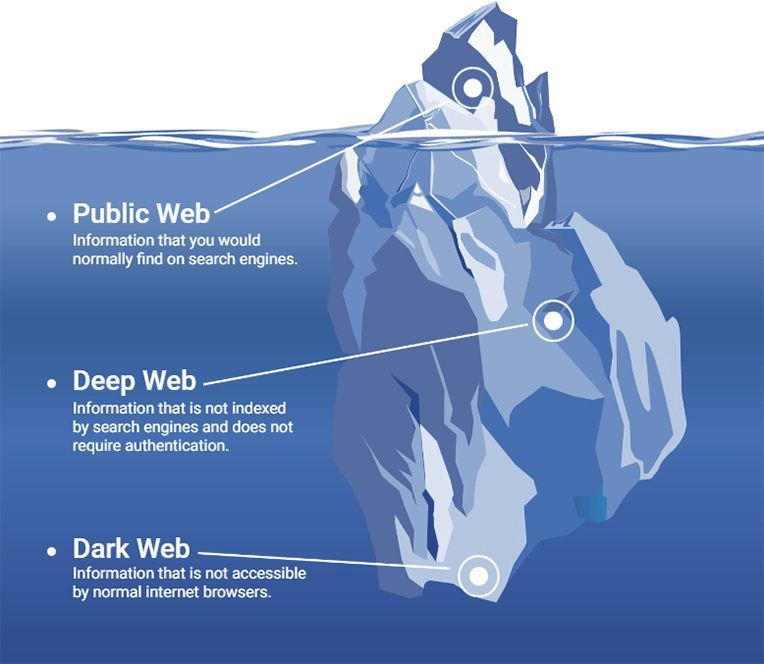
\includegraphics[width=0.8\paperwidth]{DarkNet}\hfil}}	
	}%
\begin{frame}
	\frametitle{What is the DarkNet}
	% When presenting some examples might be in order
\end{frame}
}
\begin{frame}
	\frametitle{Data - existing and gathered}
	\begin{itemize}
		\item DUTA-10K, illegal vs. legal drugs (Al Nabki et al. 2019)
		\item Manually acquired eBay products of drugs weed etc.
	\end{itemize}
\end{frame}

\begin{frame}
	\frametitle{Domain - Vocabulary}
	Jensen-Shannon divergence and Variational distance between word frequencies.
	Self distances are small while pair distances in Legal-Illegal-eBay are high.
	
	Legal and Illegal should be considered different domains, despite being both DarkNet material.
	\begin{figure}
		\centering
		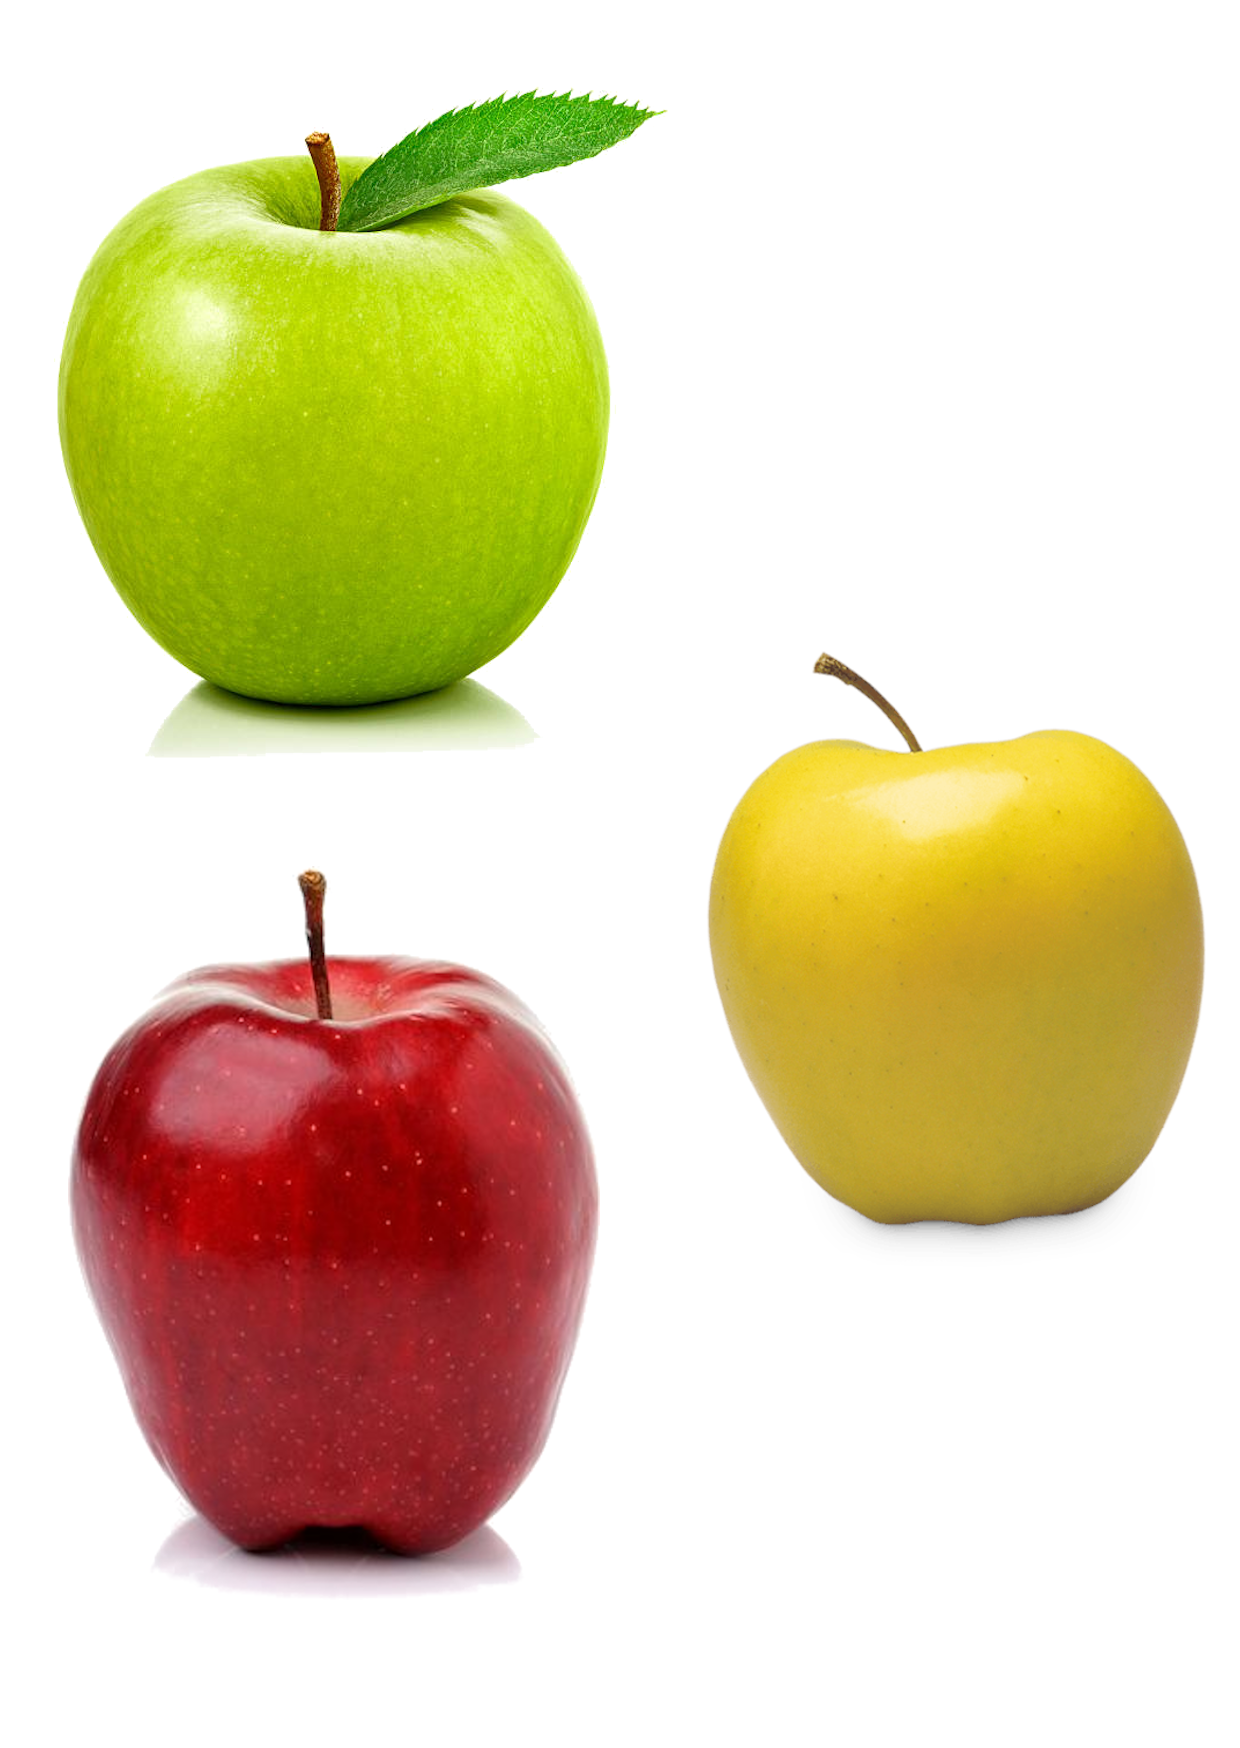
\includegraphics[width=0.3\textwidth]{3different.png}
	\end{figure}

\end{frame}

\begin{frame}
	\frametitle{Domain - NER}
\end{frame}

\begin{frame}
	\frametitle{Classification - models}
\end{frame}
\begin{frame}
	\frametitle{Classification - conditions}
	pos instead of
	dropped 
	...
\end{frame}

\begin{frame}
	\frametitle{legal DarkNet vs. eBay}
\end{frame}
\begin{frame}
	\frametitle{legal Drugs vs. illegal}
\end{frame}
\begin{frame}
	\frametitle{cross domain illegality}
\end{frame}
\section*{}

\begin{frame}
\frametitle{Conclusion}
\end{frame}

\begin{frame}[allowframebreaks]
\frametitle{References}
\bibliographystyle{apalike}
\tiny\bibliography{acl2019}
\end{frame}

\end{document}
